\paragraph{QuizziPedia::Front-End::Views::EditorQMLView}
\begin{figure} [ht]
	\centering
	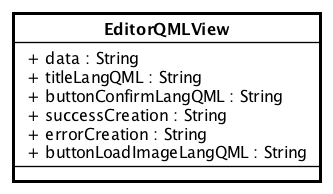
\includegraphics[scale=0.80]{UML/Classi/Front-End/QuizziPedia_Front-end_EditorQMLView.png}
	\caption{QuizziPedia::Front-End::Views::EditorQMLView}
\end{figure} \FloatBarrier
\begin{itemize}
	\item \textbf{Descrizione}: \textit{view\ped{G}} contenente l'\textit{editor\ped{G}} \textit{QML\ped{G}} per la creazione di domande personalizzate;
	\item \textbf{Utilizzo}: permette ad un utente di creare domande personalizzate attraverso la scrittura del codice \textit{QML\ped{G}} direttamente nell'\textit{editor\ped{G}} di testo presente nella \textit{view\ped{G}};
	\item \textbf{Relazioni con altre classi}:
	\begin{itemize}
		\item \textbf{IN \texttt{EditorQMLModelView}}: classe di tipo modelview la cui istanziazione è contenuta all'interno della variabile di ambiente \texttt{\$scope} di \textit{Angular\ped{G}}. All'interno di essa sono presenti le variabili e i metodi necessari per il \textit{Two-Way Data-Binding\ped{G}} tra la \textit{view\ped{G}} \texttt{EditorQMLView} e il \textit{controller\ped{G}} \texttt{EditorQMLController};
		\item \textbf{IN \texttt{LangModel}}: rappresenta il modello delle informazioni per la giusta traduzione dell'applicazione.
	\end{itemize}
	\item \textbf{Attributi}:
	\begin{itemize}
		\item \texttt{+ data: String} \\ Stringa contenente il testo inserito dall'utente nell'apposito \textit{Editor\ped{G}};
		\item \texttt{+ titleLangQML: String} \\ Attributo che viene utilizzato per visualizzare la giusta traduzione del titolo della pagina, in italiano o in inglese;
		\item \texttt{+ buttonConfirmLangQML: String} \\ Attributo che viene utilizzato per visualizzare la giusta traduzione della \textit{label\ped{G}} per il bottone di conferma, in italiano o in inglese;
		\item \texttt{+ buttonLoadImageLangQML: String} \\ Attributo che viene utilizzato per visualizzare la giusta traduzione della \textit{label\ped{G}} per il bottone di caricamento dell'immagine nel testo della domanda, in italiano o in inglese;
		\item \texttt{+ successCreation: String} \\ Attributo che visualizza un messaggio di conferma avvenuta creazione della domanda;
		\item \texttt{+ errorCreation: String} \\ Attributo che visualizza un messaggio d'errore per la creazione della domanda.
	\end{itemize}
\end{itemize}